
\documentclass{article}
\usepackage{csvsimple}
\usepackage{amsmath}
\usepackage{amssymb}
\usepackage{graphicx}
\usepackage{hyperref}
\usepackage{wrapfig}

\begin{document}

%insert your content here..

\section{Student content}
%\documentclass[article]{IEEEtran}
%\usepackage[utf8]{inputenc}
%\usepackage{graphicx}
%\usepackage{cite}
%\usepackage{url}

\title{Week 4. GitHub Assignment \\
\large UCCS CS 6000 Computer Science Research}
\author{Jose Luis Castanon Remy}
\date{September 2022}

%\begin{document}

\maketitle

\section{Myself}

During my experience working as a cybersecurity analyst, I have always faced different issues related to the field. I always thought no one had the interest to solve or even address these issues. Common issues that I have found while working are disinformation, disinterest, and uncontrol. This constitutes my second goal. I would love to research and solve issues within the cybersecurity field that no one is paying attention to. One of these issues is the fact that many companies that I had the opportunity to work for, all lack a proper inventory of software leading to security issues.



In addition to my goals and expectations, I consider myself to be very creative. I love to paint. I consider myself an artist in multiple disciplines. I love charcoals and pencils. I am currently learning color theory and how to paint figurines and build dioramas. Apart from my artistic face, I love biking. It is the best way for me to add cardio to my gym routine without getting bored.

I will be completing my Ph.D. in Cybersecurity.


\begin{figure}[htp]
    \centering
    
\includegraphics[width=4cm]{UCCSProfileIMG.jpg}
    \caption{An image of myself}
    \label{fig:myself}
\end{figure}


\section{Git Code}
I am currently working on a research related to security and software maintenance. It is a broad topic but I will be trying to narrow it down as I advance with my story.

Maintenance is a large part of every security team. Maintenance represented more than 50\% of the tasks and duties within the last security team I worked with. Part of the maintenance process was related to cleaning. There is a broadly known app related to cleaning called CCleaner. Cleaning helps solve issues directly linked to unused files within installation folders, cache folders, etc. CCleaner helps detect and clean up these files.

Currently, the tasks that CCleaner can perform are limited. For this reason, I have chosen the following Git repo, Winapp2, \url{https://github.com/MoscaDotTo/Winapp2}.

Winapp2 extends the cleaning routines of CCleaner. Winapp2 compiles a list of keys, as a configuration file, for CCleaner to check more applications to clean.
This is highly related to my research as I would like to build something that can map the stack of software within a computer system.
Winapp2 is not also compatible with CCleaner but with other cleaning apps like BleachBit, System Ninja, Avira System Speedup, Tron, and R-Wipe \& Clean. Winapp2 repository contains Winapp2ool, which helps maintain, manage, download and deploy Winapp2, \url{https://github.com/MoscaDotTo/Winapp2/tree/master/winapp2ool}


\section{Questions}
Please, leave your questions after this line.

You say your topic is broad so what types of softwares have you narrowed down so far? Or if you havent done anything yet to narrow that part down then have you looked at maybe different types of attacks to investigate, like maybe what is the most prominent attack among software vs effectiveness of these attacks? -Noah Rodgers
My topic is not focused specifically on finding vulnerabilities. It is more focus on the discovery part of the software itslef. This "discovery" is what I call mapping. Having a map of the software implies a better future protection.

JTs question/comments:  I think it's cool that you are looking at security from the maintenance perspective.  Was there ever a time that you were able to use this approach with success as an analyst?  What companies or organizations have you provided services for?
Yes, working as a security analyst is highly related to the maintenance perspective. You need to give guidence in most of the processes related to the security of the company. I am not allowed to speak about my clients, sorry.

\KoraComments{Do you have an example of what a map might look like?}
I do not but I think of the map as heat map or a bubble graph like map.

\bibliographystyle{IEEEtran}
\bibliography{refs}

%\end{document}

%\documentclass[article]{IEEEtran}
%\usepackage[utf8]{inputenc}
%\usepackage{graphicx}
%\usepackage{cite}
%\usepackage{url}

\title{GitHub Assignment}
\author{Noah Rodgers}
\date{September 2022}

%\begin{document}

\maketitle

\section{About Me}

Hello, my name is Noah Rodgers I am a Graduate Student in the Master of Cyber Security program at UCCS. I work at the Aerospace Corporation as an intern Cyber Specialist working with NASA and the Space Force. What I hope to gain from this course is how to properly conduct my research. As well as write my papers with the correct language and grammar. I hope this will further my research work as I start my work for Dr. Chang. I am working on disrupting satellite communications using different methods examining viability, and effectiveness. I am also hoping that this course will touch on how to write and prepare my thesis for my master’s program. Something personal about me is that I love to go sand boarding at the Great Sand dunes. I also like to long board to class from my home on sunny days although I’m not that good at it but I haven’t crashed yet, so I guess that’s a plus. I got my Bachelors in Game design and Development at UCCS and got my minor in computer science so I’ve been working on filling in the gaps for cyber security. I look forward to what this class has to offer.



\begin{figure}[!htb]
    \centering
    
\includegraphics[width=85mm, angle=90]{Me1.jpg}
    \caption{\textbf{Picture of Myself}}
    \label{fig:jamequation}
\end{figure}


\section{Git Code}
A collection of Resources for budding SAT hackers (Satellites, not the test¯\_(ツ)_/¯).

This is the basic hack a sat github repo where you can learn and train to help better security for these devices.

https://github.com/deptofdefense/hack-a-sat-library

\section{2 Questions to answer}
How different is the attack vector when facing a hacking process aiming for satellites? - Jose Remy



\bibliographystyle{IEEEtran}
\bibliography{refs}

%\end{document}

% \documentclass{article}
% \usepackage[utf8]{inputenc}
% \usepackage{graphicx}
\graphicspath{ {./images/} }
%\usepackage{hyperref}

\title{Turner  CS600}
\author{James Turner}
\date{September 2022}

%\begin{document}

\maketitle
\newpage
\section{Old Stuff from Assignment 1}
My name is James Turner and I am an active-duty Army Chief Warrant Officer 3 (CW3).  I have served a total of 17 years with 12 years as a Cyber Electromagnetic Warfare (EW) Technician.  This job field is extremely challenging because the technology in the marketplace and capabilities used by our adversaries is constantly changing.  However, it also stimulates innovation and creative thinking and is rewarding when you are part of a team that finds solutions to complex problems.

Recently, I was accepted into the Army’s Advanced Civil School (ACS) program that allows me to attend school full-time and complete a Master’s degree while on active duty.  I have been accepted at UCCS in the Cybersecurity Master of Engineering program, and I am a first term student.  I chose to study cybersecurity because my job field is closely connected with wireless applications and wireless security, and I realized that there is significant job growth in the cybersecurity field.

One of the primary outcomes that I desire from the CS6000 course is to become a more proficient writer and researcher.   I already possess some research and writing skills through my professional military education and on the job experience.  However, military style of writing differs from academia in that the military focuses on a “bottom line up front” perspective and tends to leave details out of formal documents.  I also hope to achieve a greater array of methods that help me conduct more thorough and rigorous research.

Another goal I desire from this course is to enhance my critical thinking.  The military embraces and teaches critical thinking at all levels of leadership education, but I want to gain a greater ability to analyze and test information with scientific methods.  The preponderance of my degree plan and research will be analyzing other tests and scientific data, so I want to be prepared to understand and evaluate those results.  I will need to sharpen my ability to challenge assumptions of others, including myself so that I can become a better researcher.

\begin{figure}
    \centering
    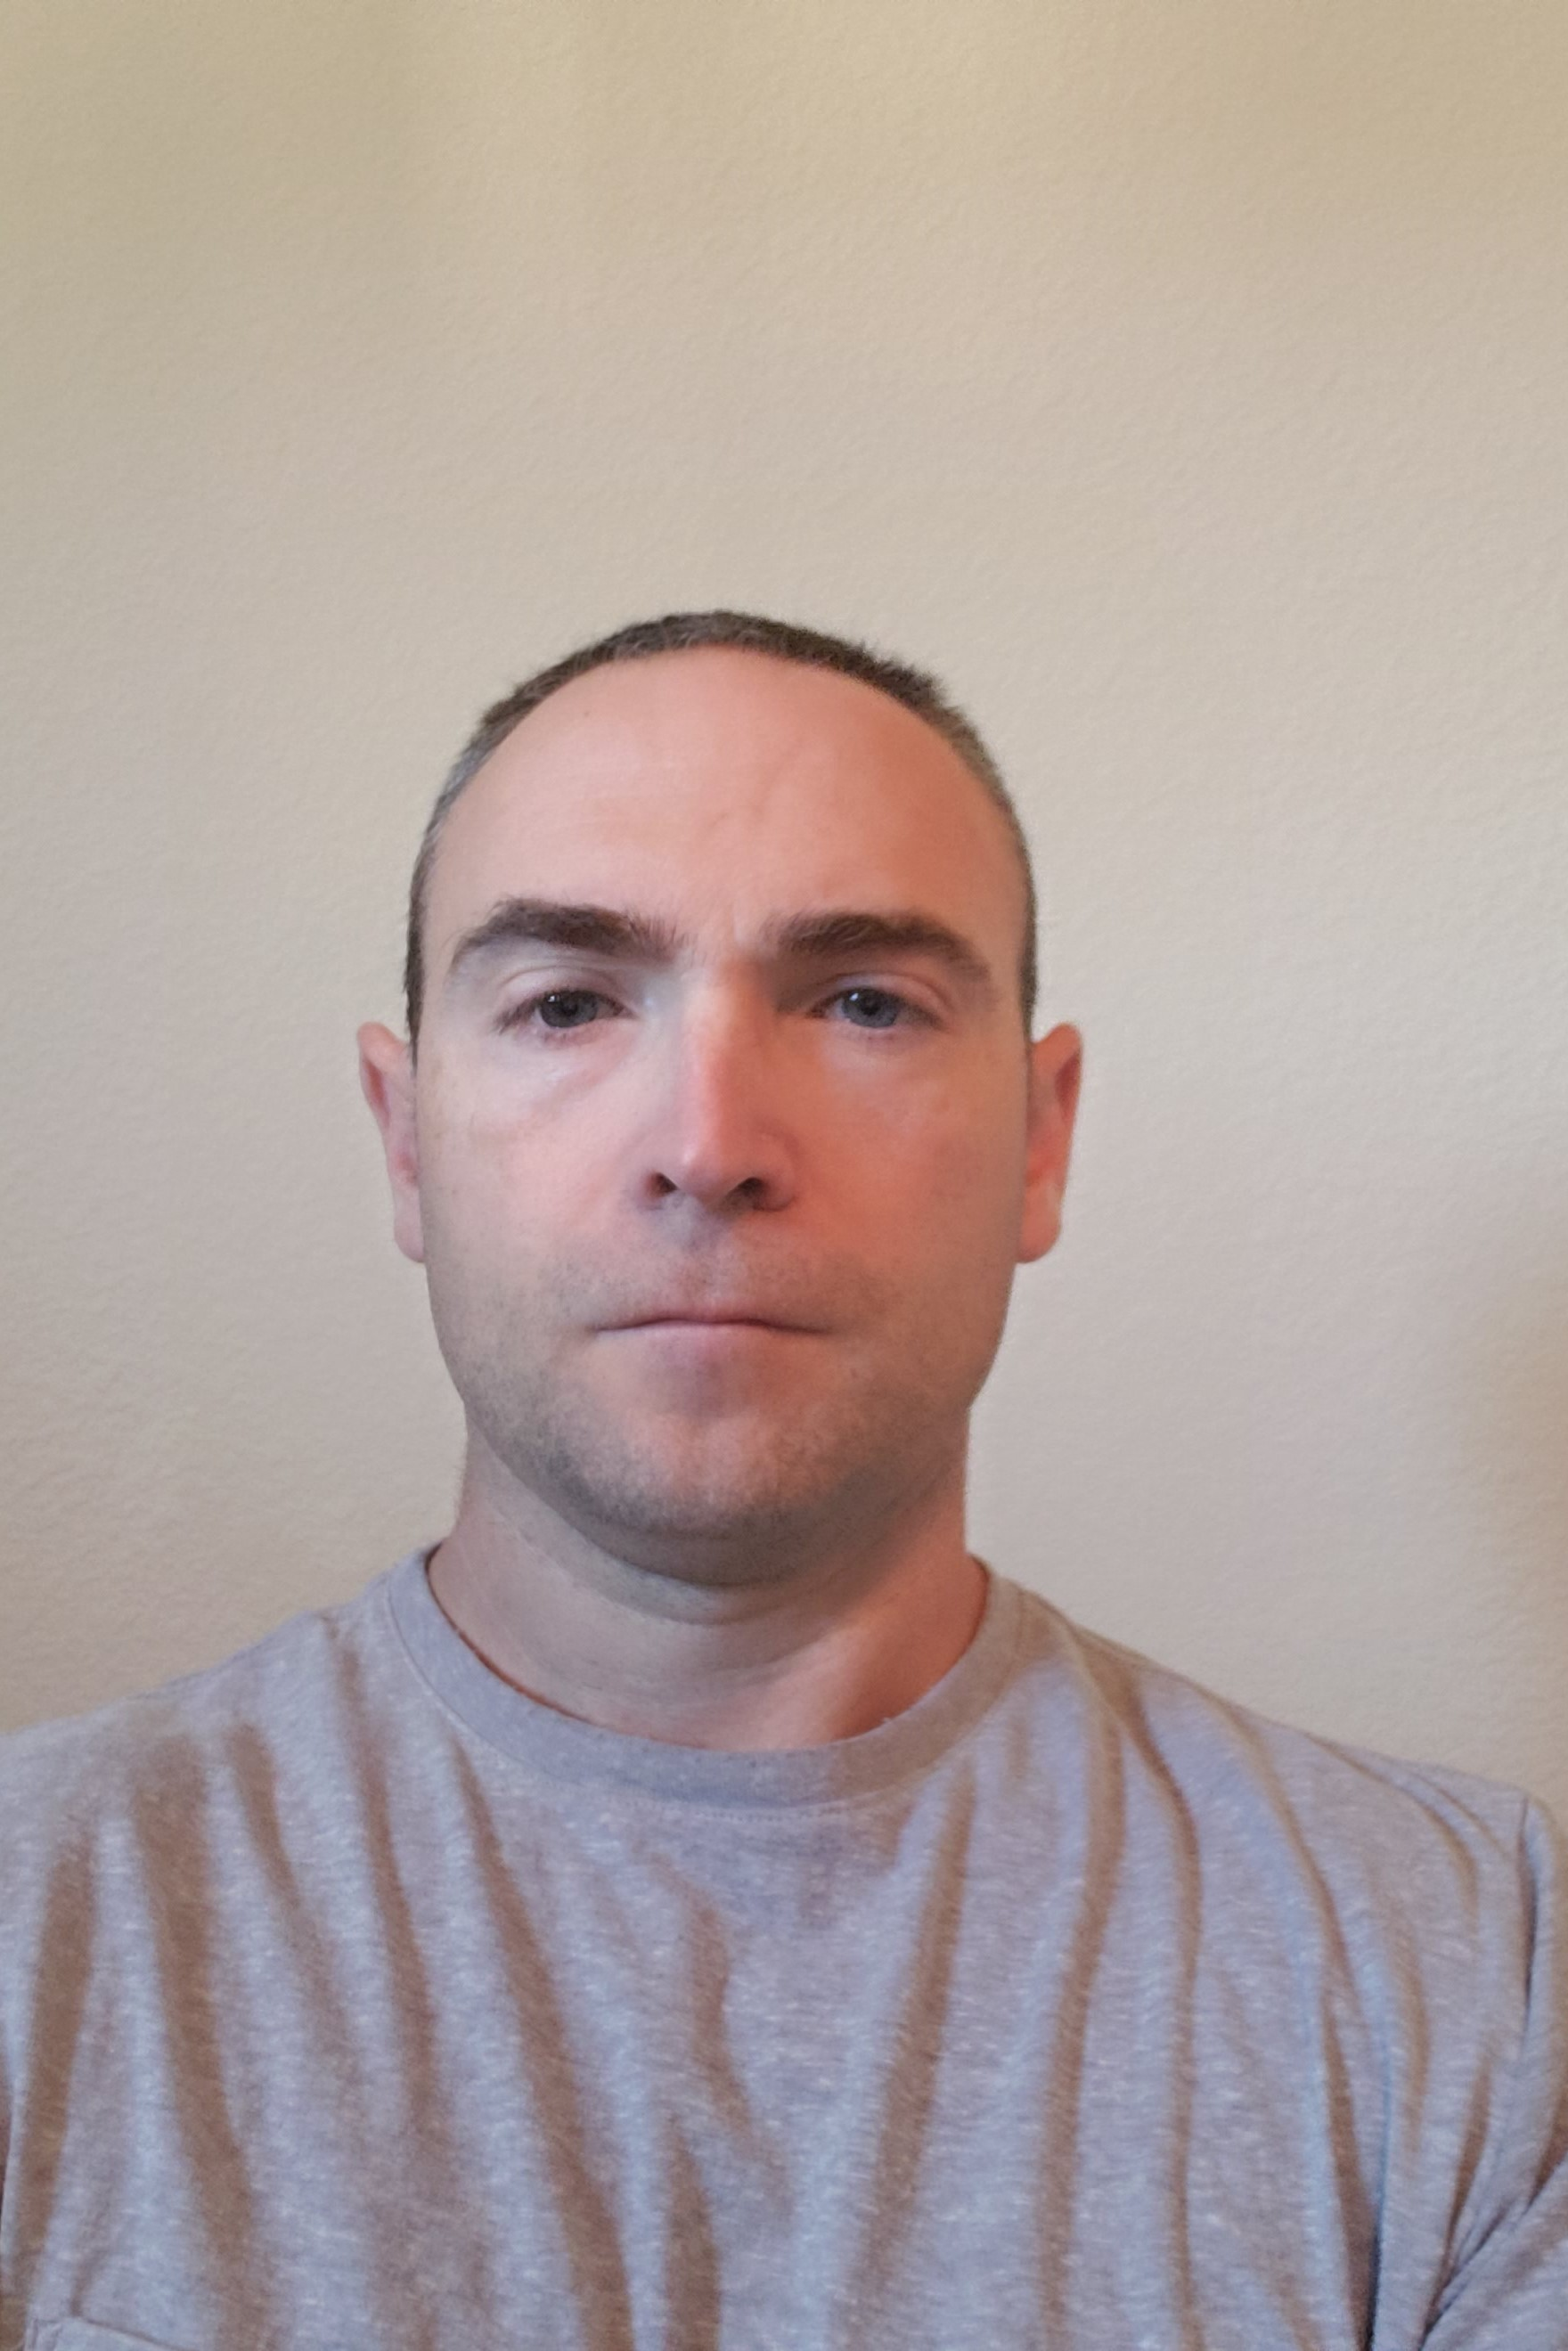
\includegraphics[scale=.1]{self pic2.jpg}
    \caption{me}
    \label{fig:me}
\end{figure}
%\newpage
\section{Github Code on Cognitive Radio}
This repository in Github contains a novel algorithm that uses linear processing to characterize the radio frequency environment in order to enable secondary users' ability to use unoccupied electromagnetic spectrum space.  The link is provided below.
\url{https://github.com/parthgargava/Cognitive-Radio-Networks}

\section{Questions}
What is the main topic that you like to work on for your master thesis, and how do you think that can benefit that army? Ali AlShami
\newline
\paragraph{}
Answer: If I still go the Thesis track then I will discuss some form of wireless security from an avaiability (redundancy and resiliency) and confidentiality perspective.  I still don't know what wireless application I will choose from.  I might focus on 5G or some new type of technology such as reconfigurable intelligent surfaces. 
\paragraph{}
Are you hoping to work on a theoretical or hands-on approach to electronic warfare? I imagine you get a fair share on hands-on experience already. -Katrina
Answer: If I can do live expirementation then that's what I will do.  Yes, I do have plenty of hands-on experiences with different forms of radios and their applications.  However, I need to get stronger from a theoretical standpoint as well.  When you play around with equipment, sometimes it's easy to lose track of the fundamentals in the design of that same equipment.

Nazmus: Have you used PKI in your research?

%\end{document}

\documentclass{article}

\usepackage[english]{babel}

\usepackage[letterpaper,top=2cm,bottom=2cm,left=3cm,right=3cm,marginparwidth=1.75cm]{geometry}


\usepackage{amsmath}
\usepackage{graphicx}
\usepackage[colorlinks=true, allcolors=blue]{hyperref}

\title{Git Assignment}
\author{Hassan Shakil}

\maketitle


\section{Introduction}

Hello, my name is Hassan shakil I am a first year Ph.D. student in UCCS. My major is Computer Science. The reason why I am taking this course in my first semester of the Ph.D. program is that after successfully completing this course I will have knowledge about computer science research and it will help in my Ph.D. degree and also I will get exposure to cutting-edge research in the field which will enable me to explore my passion and abilities. My Research interest in Text summarization using Natural Language Processing. Some personal things about me are that I was an E-sports player in my college team, I love to play and watch soccer. Moreover, I like to explore different places and go hiking.

\begin{figure}[htp]
    \centering
    
\includegraphics[width=4cm]{Myimg.jpeg}
    \caption{My picture}
    \label{fig:Myimg}
\end{figure}

\section{Git Code}
To summarize a one-page paragraph in ten sentences, researcher used the NLTK package and techniques including tokenization, stemming, lemmatization, computing similarity, and using the Page-Rank algorithm. Below is the link of git repository that has code related to text summarization.

\url{https://github.com/harshdarji23/Text-Summarization-An-Extractive-Method-NLP.git}

\section{Ask Questions}
Please ask questions here.
Hi Hassan, I'm also interested in natural language processing. Who is your Ph.D. advisor?
Hi, that's great if you are also interested in NLP. My advisor is Dr. Jugal Kalita.

\documentclass[a4paper]{article}

%% Language and font encodings
\usepackage[english]{babel}
\usepackage[T1]{fontenc}

%% Sets page size and margins
\usepackage[a4paper,top=3cm,bottom=2cm,left=3cm,right=3cm,marginparwidth=1.75cm]{geometry}

%% Useful packages
\usepackage{amsmath}
\usepackage{graphicx}
\usepackage[colorinlistoftodos]{todonotes}
\usepackage[colorlinks=true, allcolors=blue]{hyperref}

\title{Week 1 Journal}
\author{Kevin Cardenas}

\begin{document}
\maketitle

\section{Introduction and Goals for CS6000}

My name is Kevin Cardenas and I am a Captain in the US Air Force. I have the unique opportunity to be a full-time PhD student for my job as an active duty military member. I taught in the Department of Computer and Cyber Sciences at the USAF Academy for three years and will be able to go back to teaching after completing my PhD. The most challenging aspect of my PhD will be the fact that the Air Force only grants me three years to complete my degree. I chose to get a PhD in Computer Science so I could become a better asset for the USAF Academy and broaden my experience in the realm of Data Science. This will most likely add to the challenge of completing this degree in three years, but I like challenges. 

One of my primary goals for this course is to learn how to quickly sift through large volumes of articles/conference papers/journals/etc to find pertinent information relating to my area of research. A secondary goal for this course is to have a well defined research topic by the end of the semester. These two goals should help me overcome the shortened time limitation the Air Force requires to complete a PhD.

\section{Git Repo}
    \href{https://github.com/serengil/deepface}{Deepface} is a lightweight face recognition and facial attribute analysis (age, gender, emotion and race) framework for python. It is a hybrid face recognition framework wrapping state-of-the-art models: VGG-Face, Google FaceNet, OpenFace, Facebook DeepFace, DeepID, ArcFace, Dlib and SFace.

Experiments show that human beings have 97.53% accuracy on facial recognition tasks whereas those models already reached and passed that accuracy level.

\begin{figure}[!htb]
\centering

\includegraphics[width=0.4\textwidth]{figures/Kevin.jpg}
\caption{\label{fig:me}Wedding day mess dress (6 Sept 2019).}
\end{figure}

\end{document}

\section{Example of Easy Tables}
\csvautotabular{test.csv}


\section*{Better formated Tables}
    \begin{tabular}{r|r|r}%
    % specify table head
    \bf Time (s) & \bf Rel. time (s)& \bf Y Pos
% use head of csv as column names
    \csvreader{test.csv}{}
% specify selected coloumns here
    {\\\hline\csvcoli&\csvcolii&\csvcolvi}
    \end{tabular}
    \clearpage


\end{document}
